% SC3270 --- Chapter 1: What Correct Means and Hoare Triples (0->100 ground-up)
\chapter{What Correct Means and Hoare Triples}
\label{ch:hoare-intro}

\begin{quote}
\emph{``A program is correct not when it passes ten tests, but when no test could make it fail.''} We move from sampling behaviours (testing) to quantifying over all behaviours (proof).
\end{quote}

\noindent\fbox{\parbox{\dimexpr\linewidth-2\fboxsep-2\fboxrule}{%
\textbf{From zero: no verification background assumed.} We define what a program does via its states, build up what an assertion means, and introduce Hoare triples as contracts. Pictures come first; every formal rule is motivated by a tiny program you can run. Only basic programming and high-school logic are assumed.}}
\vspace{0.4em}

\section*{Learning Outcomes}
After this chapter you will be able to:
\begin{enumerate}[label=(L\arabic*)]
    \item define program state and assertion as a set of states;
    \item write a Hoare triple $\{P\}\,C\,\{Q\}$ and read its meaning;
    \item distinguish partial correctness from total correctness;
    \item explain why testing can miss bugs that proof must cover;
    \item state the intuitive meaning of consequence and composition.
\end{enumerate}

% ============================================================
\section{Why Testing Is Not Enough}
\label{sec:testing-vs-proof}
\paragraph{Intuition.} Think of a program as a machine that reads a suitcase of variables $\{x,y,\dots\}$ and transforms it. The suitcase contents is the \emph{state}. Testing opens the machine on ten suitcases and checks the outputs. Proof asks: does the machine do the right thing on \emph{every} suitcase that satisfies the boarding condition?

Consider absolute value:
\begin{center}
\texttt{if x < 0 then x := -x}
\end{center}
Testing $x=2$ and $x=-3$ succeeds. Yet $x=-2^{31}$ on 32-bit two's complement overflows. A proof quantifies over all $x$.

\begin{figure}[h]\centering
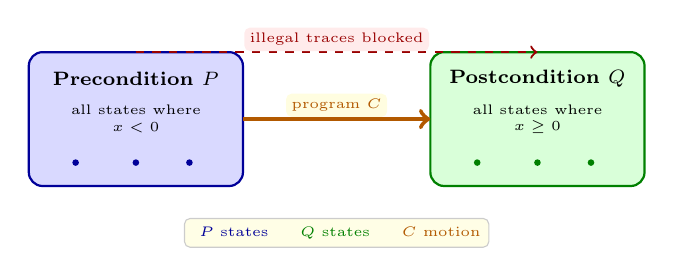
\begin{tikzpicture}[scale=0.85,font=\scriptsize]
\draw[fill=blue!15,draw=blue!60!black,thick,rounded corners=5pt] (0,0) rectangle (3.2,2.0);
\node at (1.6,1.6) {\textbf{Precondition $P$}};
\node[font=\tiny,align=center] at (1.6,1.0) {all states where\\ $x < 0$};
\draw[fill=green!15,draw=green!50!black,thick,rounded corners=5pt] (6.0,0) rectangle (9.2,2.0);
\node at (7.6,1.6) {\textbf{Postcondition $Q$}};
\node[font=\tiny,align=center] at (7.6,1.0) {all states where\\ $x \ge 0$};
\draw[->,ultra thick,orange!70!black] (3.2,1.0) -- (6.0,1.0) node[midway,above,font=\tiny,fill=yellow!12,rounded corners=2pt,inner sep=2pt] {program $C$};
\foreach \x in {0.7,1.6,2.4} \fill[blue!60!black] (\x,0.35) circle (1.4pt);
\foreach \x in {6.7,7.6,8.4} \fill[green!50!black] (\x,0.35) circle (1.4pt);
\draw[->,thick,red!60!black,dashed] (1.6,2.0) -- (7.6,2.0) node[midway,above,font=\tiny,fill=red!08,rounded corners=2pt,inner sep=2pt] {illegal traces blocked};
\node[font=\tiny,align=left,fill=yellow!10,draw=gray!40,rounded corners=2pt,inner sep=3pt] at (4.6,-0.70) {\textcolor{blue!60!black}{$\blacksquare$ $P$ states} \quad \textcolor{green!50!black}{$\blacksquare$ $Q$ states} \quad \textcolor{orange!70!black}{$\blacksquare$ $C$ motion}};
\end{tikzpicture}
\caption{A Hoare triple $\{P\}\,C\,\{Q\}$: every $P$-state moved by $C$ must land in $Q$. The program is a conveyor from the blue set to the green set.}
\label{fig:triple-conveyor}
\end{figure}

\begin{figure}[h]\centering
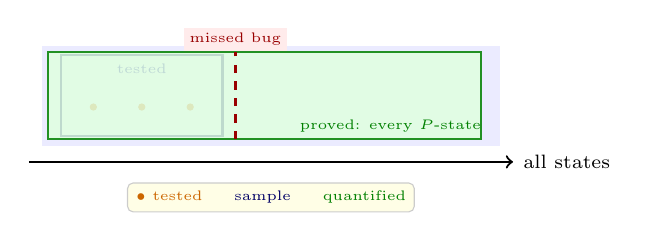
\begin{tikzpicture}[scale=0.82,font=\scriptsize]
\draw[->,thick] (0,0) -- (7.5,0) node[right] {all states};
\fill[blue!08] (0.2,0.25) rectangle (7.3,1.8);
\draw[thick,blue!40!black] (0.5,0.40) rectangle (3.0,1.65);
\node[font=\tiny,blue!60!black] at (1.75,1.45) {tested};
\foreach \x in {1.0,1.75,2.5} \fill[orange!80!black] (\x,0.85) circle (1.6pt);
\draw[thick,green!50!black,fill=green!12,opacity=0.85] (0.30,0.35) rectangle (7.0,1.70);
\node[font=\tiny,green!50!black] at (5.6,0.55) {proved: every $P$-state};
\draw[thick,red!60!black,dashed] (3.2,0.35) -- (3.2,1.70) node[above,font=\tiny,fill=red!08,inner sep=2pt] {missed bug};
\node[font=\tiny,align=left,fill=yellow!10,draw=gray!40,rounded corners=2pt,inner sep=3pt] at (3.75,-0.55) {\textcolor{orange!80!black}{$\bullet$ tested} \quad \textcolor{blue!40!black}{$\square$ sample} \quad \textcolor{green!50!black}{$\square$ quantified}};
\end{tikzpicture}
\caption{Testing samples finitely many points (orange dots) inside the blue sample box; proof shades the entire green region. A bug lurking outside the sample is invisible to tests but caught by proof.}
\label{fig:test-vs-proof}
\end{figure}

% ============================================================
\section{States, Assertions, Triples}
\label{sec:states}
\begin{definition}[State and assertion]
A \emph{state} $\sigma$ is a mapping from variables to values, e.g.\ $\{x\mapsto 3,y\mapsto -1\}$. An \emph{assertion} $P$ is a logical formula over program variables; it denotes the \emph{set} of states where $P$ holds: $\llbracket P\rrbracket=\{\sigma\mid \sigma\models P\}$.
\end{definition}

So $x>0$ is not a boolean computed by the program—it is a \emph{description} of infinitely many states. Writing $x=y+1$ means the set where the equation holds.

\begin{definition}[Hoare triple]
$\{P\}\,C\,\{Q\}$ means: if $C$ starts in any state satisfying $P$ and $C$ terminates, then the final state satisfies $Q$. This is \emph{partial} correctness—it says nothing if $C$ loops forever. \emph{Total} correctness $[P]\,C\,[Q]$ additionally requires termination.
\end{definition}

Example: $\{ \text{true}\}\; x:=x+1\; \{x>0\}$ is false (start $x=-5$, end $-4$). $\{x>0\}\; x:=x+1\; \{x>1\}$ is true. Formally, $\{P\}\,C\,\{Q\}$ is a specification; $C$ is an implementation. The triple is the \emph{conveyor} picture: $P$ states ride $C$ and must arrive in $Q$.

\begin{lstlisting}[language=Python, caption={Assertions as runtime checks: the idea behind Hoare triples made executable.}, label={lst:assert-py}]
# Assertion as set of states: we test membership by evaluating a formula
def triple_holds(P, C, Q, states):
    """Check {P} C {Q} by brute force on a finite sample of states."""
    for s in states:
        if P(s):               # only P-states matter
            s2 = C(s.copy())   # run C
            if s2 is not None and not Q(s2):
                return False, s, s2  # counterexample: P held, Q failed
    return True, None, None

# Example: absolute value program
def C_abs(s): 
    if s['x'] < 0: s['x'] = -s['x']
    return s

P = lambda s: True             # any starting state
Q = lambda s: s['x'] >= 0      # must be non-negative afterwards
print(triple_holds(P, C_abs, Q, [{'x':v} for v in [-3,0,2,5]]))
\end{lstlisting}

% ============================================================
\section{A First Proof Without Machinery}
\label{sec:first-proof}
Take $C\equiv x:=x+1;\; y:=2*x$ with spec $\{x=3\}\;C\;\{y=8\}$. Informally: after $x:=x+1$, we know $x=4$; then $y:=2*x$ gives $y=8$. That two-step chain already uses the deepest Hoare ideas: assignment as substitution and sequencing as composition. We will formalise them as axioms in Chapter~2; for now see the pattern.

\begin{figure}[h]\centering
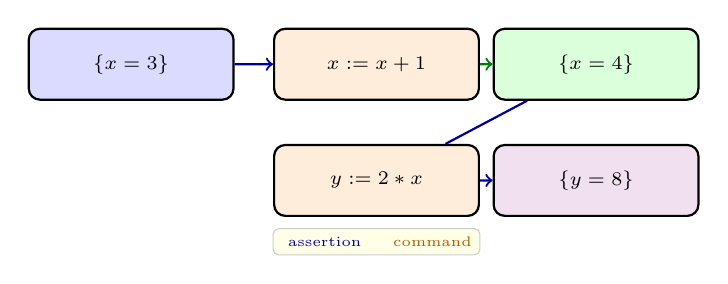
\begin{tikzpicture}[scale=0.82,font=\scriptsize,
  box/.style={draw,thick,rounded corners=4pt,align=center,minimum width=2.6cm,minimum height=0.9cm}]
\node[box,fill=blue!14] (p) at (0,1.2) {$\{x=3\}$};
\node[box,fill=orange!14] (c1) at (3.8,1.2) {$x:=x+1$};
\node[box,fill=green!14] (mid) at (7.2,1.2) {$\{x=4\}$};
\node[box,fill=orange!14] (c2) at (3.8,-0.6) {$y:=2*x$};
\node[box,fill=violet!12] (q) at (7.2,-0.6) {$\{y=8\}$};
\draw[->,thick,blue!60!black] (p) -- (c1);
\draw[->,thick,green!50!black] (c1) -- (mid);
\draw[->,thick,blue!60!black] (mid) -- (c2) -- (q);
\node[font=\tiny,fill=yellow!10,draw=gray!40,rounded corners=2pt,inner sep=3pt] at (3.8,-1.55) {\textcolor{blue!60!black}{$\blacksquare$ assertion} \quad \textcolor{orange!70!black}{$\blacksquare$ command}};
\end{tikzpicture}
\caption{Sequencing as a conveyor: the intermediate assertion $\{x=4\}$ is the handoff point between two assignments.}
\label{fig:seq-conveyor}
\end{figure}

\begin{lstlisting}[language=C, caption={Same idea in C: pre/post as comments. The proof obligation is that no $P$-state escapes to $\neg Q$.}, label={lst:triple-c}]
// { x == 3 }   <-- P holds before
x = x + 1;      // now { x == 4 } must hold (assignment axiom preview)
// { x == 4 }
y = 2 * x;      // now { y == 8 } must hold
// { y == 8 }   <-- Q holds after, if we terminate
\end{lstlisting}

Partial vs.\ total: $\{x\ge 0\}\;\texttt{while }x>0\;\texttt{do }x:=x-1\;\{x=0\}$ is true for partial correctness (if it stops, $x=0$). It is also totally correct because the loop always stops—Chapter~6 will prove it. But $\{ \text{true}\}\;\texttt{while true do skip}\;\{ \text{false}\}$ is vacuously partially correct (it never terminates, so the ``if it terminates'' is empty), yet not totally correct.

\begin{remark}[Vacuous truth]
$\{ \text{false}\}\,C\,\{Q\}$ is always true: there is no $P$-state to check. This mirrors ``if false then anything'' and explains why an impossible precondition makes any spec trivially hold—watch for it when you strengthen preconditions too far.
\end{remark}

% ============================================================
\section{Consequence: Strengthening and Weakening}
\label{sec:consequence}
\paragraph{Intuition.} If you prove $\{P\}\,C\,\{Q\}$ and you know $P' \Rightarrow P$ (so $P'$ is smaller, stronger), then $\{P'\}\,C\,\{Q\}$ is free: every $P'$-state is already a $P$-state. Dually, if $Q \Rightarrow Q'$ (so $Q'$ is larger, weaker), then $\{P\}\,C\,\{Q'\}$ follows—landing in $Q$ guarantees landing in the bigger set $Q'$.

Think of sets. Let $\llbracket P'\rrbracket \subseteq \llbracket P\rrbracket$ and $\llbracket Q\rrbracket \subseteq \llbracket Q'\rrbracket$. The triple says the image of $\llbracket P\rrbracket$ under $C$ sits inside $\llbracket Q\rrbracket$. Then the image of the smaller $\llbracket P'\rrbracket$ sits inside $\llbracket Q\rrbracket \subseteq \llbracket Q'\rrbracket$. No re-proof of $C$ needed.

Formally this is the rule of \emph{consequence}; Chapter~2 makes it an inference rule:
\[
\frac{P' \Rightarrow P \quad \{P\}\,C\,\{Q\} \quad Q \Rightarrow Q'}{\{P'\}\,C\,\{Q'\}}.
\]
It is the workhorse for fitting a proven triple to the pre/post your caller actually has.

\begin{example}[Consequence in use]
We prove $\{x=3\}\,x:=x+1\,\{x=4\}$. A caller has $\{x=3 \land y=0\}$. Since $(x=3\land y=0)\Rightarrow (x=3)$, consequence gives $\{x=3\land y=0\}\,x:=x+1\,\{x=4\}$. Then weaken $x=4 \Rightarrow x>0$ to obtain $\{x=3\land y=0\}\,x:=x+1\,\{x>0\}$. The program did not change; our description did.
\end{example}

% ============================================================
\section{Worked Example: Specifying Maximum}
\label{sec:max-example}
Specify $m:=\text{if }a\ge b\text{ then }a\text{ else }b$ so that $m$ is the maximum. Attempt 1: $\{ \text{true}\}\,C\,\{m\ge a \land m\ge b\}$ is true but too weak—it allows $m=100$ when $a=2,b=3$. We need ``$m$ equals one of the inputs and dominates both'':
\[
\{ \text{true}\}\; C\; \{ (m=a \lor m=b)\ \land\ m\ge a\ \land\ m\ge b\}.
\]
Equivalently $m=\max(a,b)$. The disjunction is essential because we do not know statically which branch runs.

Why not $\{a\ge b\}\,C\,\{m=a\}$? That is true but incomplete—it only handles half the inputs. The full spec with $\text{true}$ as pre forces the program to handle both branches, and the proof must case-split on $a\ge b$.

This pattern recurs: a precise postcondition often needs $\lor$, $\exists$, or quantifiers to describe ``whichever path was taken, the output has this shape.'' Vague posts give vacuous proofs.

\begin{remark}[Contracts as promises]
A triple is a \emph{contract}: the caller promises to establish $P$; the callee promises to establish $Q$ if it terminates. This is identical to JML's \texttt{requires/ensures} or Eiffel's \texttt{pre/post} that you will write in Chapter~3. The proof is the evidence that the promise is kept for all admissible callers.
\end{remark}

% ============================================================
\section{What Partial Leaves Out: Preview of Termination}
\label{sec:partial-total-preview}
Partial correctness guarantees ``if you finish, you finish right'' but never promises finishing. The classic villain is a loop that never makes progress:
\begin{center}
\texttt{while x > 0 do x := x} \quad---\, $x$ never changes, so $\{x\ge0\}\,C\,\{x=0\}$ is partially correct (vacuously when $x>0$, because it never exits), yet totally false.
\end{center}
Dijkstra called this the ``fire alarm'' problem: a program that burns forever still satisfies every partial spec. Chapter~6 adds \emph{variants} to rule it out. For now remember: total correctness $=$ partial $+$ termination, and the two concerns need different proof tools (invariants vs.\ ranking functions).

\begin{example}[Absolute value total]
$\{\text{true}\}\;\texttt{if }x<0\texttt{ then }x:=-x\;\{x\ge0\}$ is both partially and totally correct: the program has no loops, so termination is trivial. Contrast $\{\text{true}\}\;\texttt{while }x<0\texttt{ do }x:=x+1\;\{x\ge0\}$—partially correct (if it stops, $x\ge0$), but totally correct only when $x$ is bounded above; we must exhibit a variant $-x$ that decreases.
\end{example}

% ============================================================
\section{Exercises}
\label{sec:ch01-exercises}
\begin{enumerate}[label=E1.\arabic*, leftmargin=*, itemsep=0.6em]
    \item \textbf{State sets.} Write the set $\llbracket x>0\land y=x+1\rrbracket$ informally. Give two states inside and two outside. Why is an assertion a set, not a single state?
    \item \textbf{True or false triples.} Decide for each: (a) $\{x=5\}\,x:=x+1\,\{x=6\}$, (b) $\{x>0\}\,x:=x-1\,\{x\ge0\}$, (c) $\{ \text{true}\}\,\texttt{while true do skip}\,\{\text{false}\}$ for partial correctness. Justify.
    \item \textbf{Max spec.} Write a Hoare triple for $m:=\max(a,b)$ using $\{ \text{true}\}$ as pre and a post with disjunction. Why is disjunction needed?
    \item \textbf{Testing blind spot.} Give a program where testing 100 random states all satisfy $\{P\}\,C\,\{Q\}$ yet the triple is false. Exhibit the counterexample state and explain why random sampling missed it logically.
    \item \textbf{Partial vs total.} State $\{n\ge0\}\,\texttt{while }n>0\texttt{ do }n:=n-1\,\{n=0\}$ in both partial and total form. Which extra obligation does total add, and why is it non-trivial?
\end{enumerate}

\section*{Chapter Notes}
Hoare's 1969 paper ``An Axiomatic Basis for Computer Programming'' introduced triples. Partial vs.\ total correctness is Floyd/Hoare; Manna--Waldinger and Winskel give gentle introductions. The conveyor picture is standard in Pierce's \emph{Software Foundations}, Vol.~1, Ch.~Hoare. For a historical view see Jones, ``The Early Search for Tractable Ways of Reasoning About Programs.''

\smallskip
\begin{remark}[How to read the rest of this book]
Each chapter follows intuition $\to$ formal $\to$ example $\to$ exercise. Run every listing, draw every diagram on paper, and instantiate each triple with two concrete states—one that should be accepted and one rejected. That habit turns abstract logic into debugging skill.
\end{remark}
% End of Chapter 1
